\section*{Lectura 1: La Teorema de Puntos Fijos de Brouwer.}

Empezamos con declara notaci\'on Vamos a denotar las siguentes conjuntos:

\begin{definition}
    Denotamos la \textbf{$n$-esfera} como el conjuno $S^n=\{x \in
    \R^{n+1} : \|x\|=1\}$ y la \textbf{$n$-bola} como el conjunto $D^n=\{x
    \in \R^{n} : \|x\| \leq 1\}$, donde $\|\cdot\|$ el la \textbf{norma} en
    $\R^n$ que induca la topolog\'ia usual de $\R^n$. Llamamos punto
    $N=(0,\dots,0,1)$ de $S^n$ el \textbf{polo norte} de $s^n$ y el punto $S=(0,
    \dots, -1)$ de $S_n$ el  \textbf{polo sur} de $S^n$. Definimos la
    \textbf{ecuador} de una $n+1$-esfera $S^{n+1}$ de ser la $n$-esfera $S^n$.
\end{definition}

\begin{example}\label{exmp_1}
    \begin{enumerate}
        \item[(1)] $S^1$ es el circulo unitario en el plano $\R^2$, y  $S^2$ es
            el esfera unitario en el espacio $\R^3$.

        \item[(2)] Nota que $S^0=\{-1,1\}$ es la unica esfera no conexo en $\R$.

        \item[(3)] Toda $n$-esfera tiene un polo norte y un polo sur. De hecho,
            el polo norte de $S^0$ es $1$ y el polo sur es $-1$.

        \item[(4)] Nota que el borde de una $n$-bola es una  $n$-esfera. Es
            decie  $\partial{D^n}=S^{n-1}$.
    \end{enumerate}
\end{example}

\begin{definition}
    Denotamos una \textbf{$n$-simplejo est\'andar} de $\R^n$ de ser el conjunto
    $\Delta^n=\{x \in \R^{n+1} : x_i \geq 0 \text{ y } \sum{x_i}=1\}$.
\end{definition}

\begin{example}\label{exmp_2}
    \begin{enumerate}
        \item[(1)] $\Delta^0=\{1\} \subeteq \R$.

        \item[(2)] $\Delta^1$ es una recta entre los puntos $(0,1)$ y $(1,0)$ en
            $\R^2$ restrinjido a la primera caudrante.

        \item[(3)] $\Delta^2$ es una tetrahedro en la primer oct\'ante de  $\R$
            con vertices en  $(0,0,1)$, $(0,1,0)$, y $(1,0,0)$. Se representa en
            la figura \ref{fig_1} tambi\'en.

        \item[(4)] Note que $\Delta^0 \subseteq \Delta^1 \leq \Delta^2$.

        \item[(5)] Como espacions topologicos, se puede demostrar que los
            $n$-simplejos est\'andares son homeomorfo a los  $n$-bolas. Es decir
             $\Delta^n \simeq D^n$.
    \end{enumerate}
\end{example}

\begin{figure}[h]
    \centering
    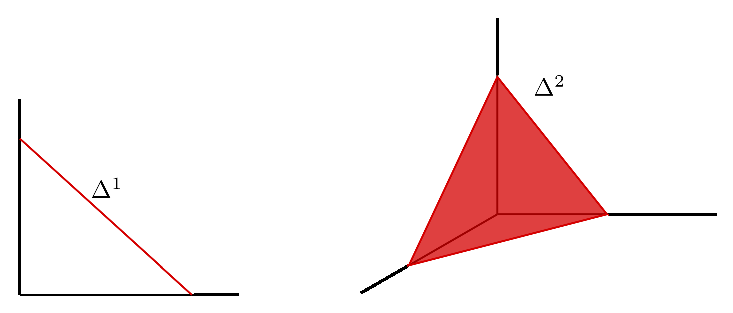
\includegraphics[scale=0.5]{Figures/standaard_simplices.eps}
    \caption{El $1$-simplejo y  $2$-simplejo est\'anderes.}
    \label{fig_1}
\end{figure}

\begin{definition}
    Sea $f:A \rightarrow A$ una funci\'on. Llamamos u punto $x \in A$ un
    \textbf{punto fijo} si $f(x)=x$.
\end{definition}

\begin{theorem}[Teorema de Puntos Fijos de Brouwer]\label{thm_1}
    S\'i $f:D^n \rightarrow D^n$ es una funci\'on continua, entonces existe un
    punto fijo en $D^n$ para toda $n \geq 1$.
\end{theorem}
\begin{proof}
    Demostramos la teorema para $n=1$. Es decir, que toda funci\'on  $f:B^1
    \rightarrow B^1$ tiene un punto fijo. Sean $a=f(-1)$ y $b=f(1)$. S\'i $a=-1$ o
    $b=1$, tenemos puntos fijos y terminamos.

    Ahora, considere la gr\'afica de $f$,  $G_f=\{(x,f(x)) : x \in B^1\}$, la
    diagonal de $B^1$, $\Delta(B^1)=\{(x,x) : x \in B^1\}$, y los medio planos
    $H^+_\Delta=\{(x,y) : y>x\}$ y $H^-_\Delta=\{(x,y) : y<x\}$. Nota que
    $\Delta(B^1)$ es la grafica de la recta $y=x$ restringido a $B^1 \times B^1$.
    Ahora, defina conjuntos
    \begin{align*}
        A   &=      \{(x,f(x)) : f(x)>x\} \\
        B   &=      \{(x,f(x)) : f(x)<x\} \\
        C   &=      \{(x,f(x)) : f(x)=x\} \\
    \end{align*}
    Entonces $C$ es el conjunto de puntos fijos de $f$. Nota que $A \subseteq
    H^+_\Delta$,  $B \subseteq H^-_\Delta$, y $C \subseteq \Delta(B^1)$. Tambien
    nota que los medio planos son abiertos en
    $\R^2$. Ahora, como  $B^1$ es compacto, y Hausdorff, se puede demostrar que
    $G_f$ y  $\Delta(B^1)$ son cerrados. Se puede ver la grafica de $f$ en el
    figura \ref{fig_2}

    Ahora, not que $G_f$ es conexo ya que es la imagen de la funci\'on $i_{B^1}
    \times f$. Como  $f$ y  $i_{B^1}$ son continua, entonces  $i_{B^1} \times f$
    es continua. Entonces como  $B^1$ es conexo, entonces $i_{B^1} \times
    f(B^1)=B^1 \times B^1$ es conexo. Ahora, nota que $G_f=A \cup B \cup C$.
    Suponga que $C=\emptyset$. Entonces  $G_f=A \cup B$. Pero tenemos que $A
    \subseteq H^+_\Delta$, y $B \subseteq H^-_\Delta$, por lo tanto, $A$ y  $B$
    son conjuntos abiertos, y que  $A$  y $B$ son disjuntos. Por lo tanto $A \cup
    B$ es una separaci\'on abierta de  $G_f$, una contradicci\'on. Por lo tanto
    $C \neq \emptyset$ y existe puntos fijos de  $f$ para $n=1$.
\end{proof}
\begin{remark}
    Para $n > 1$ no se ha encontrado una demostraci\'on general del teorema de
    puntos fijos. De hecho, es muy dificil para demostrar en general. Pero, se
    puede usar la maquinaria de la topologi\'ia algebraica para construir un
    bosquejo de una demostraci\'on.
\end{remark}

\begin{figure}[h]
    \centering
    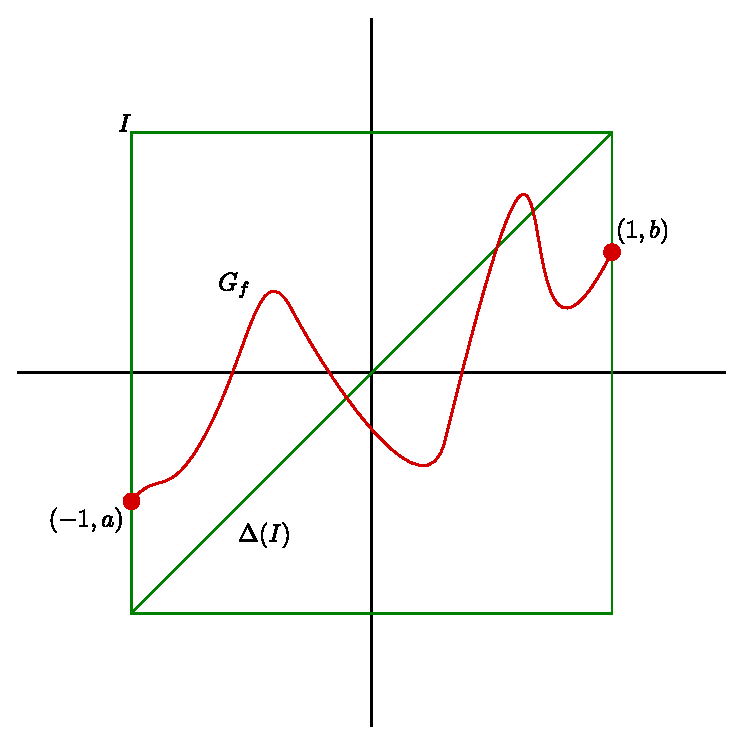
\includegraphics[scale=0.8]{Figures/brouwers_thm_1.eps}
    \caption{Demostraci\'on del teorema de puntos fijos de Brouwer.}
    \label{fig_2}
\end{figure}
